\section{Multiword division}
\subsection{Aim}
To divide a 32 bit number with a 16 bit number

\subsection{Code}
\begin{lstlisting}
DATA SEGMENT
	dividend DD 1000000H
	divisor DW 1000H
	quotient DD ?
	remainder DD ?
ENDS DATA

CODE SEGMENT
ASSUME CS:CODE, DS:DATA 
START:
	MOV AX, DATA
	MOV DS, AX
	MOV AX, WORD PTR [dividend+2]
	MOV BX, WORD PTR [divisor]
	DIV BX
	MOV WORD PTR [quotient+2], AX
	MOV AX, WORD PTR [dividend]
	DIV BX
	MOV WORD PTR [quotient], AX
	MOV WORD PTR [remainder], DX
	MOV AH, 04CH
    INT 21H
ENDS CODE
END START
\end{lstlisting}

\subsection{Output}
\begin{center}
	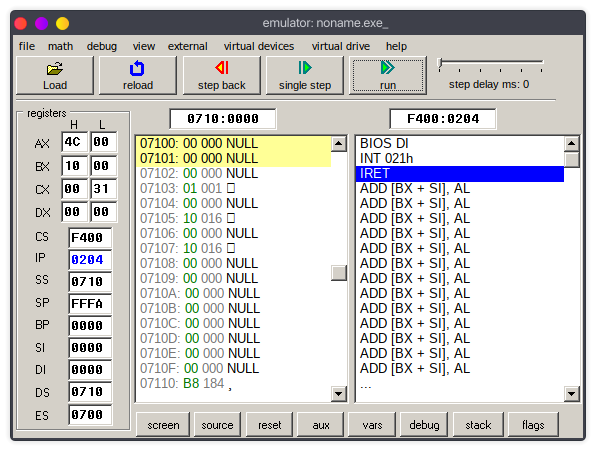
\includegraphics[width=0.90\textwidth]{img/p6/ss1.png}
	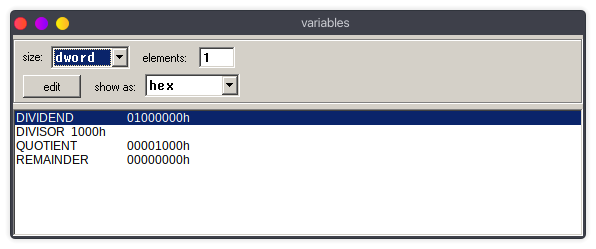
\includegraphics[width=0.90\textwidth]{img/p6/ss2.png}
\end{center}

\subsection{Result}
A 32 bit number was divided by a 16bit number in emu8086 and output was verified